\documentclass{article}
\usepackage[utf8]{inputenc}

\usepackage{ifxetex}
\ifxetex
  \usepackage{fontspec}
\else
  \usepackage[T1]{fontenc}
  \usepackage[utf8]{inputenc}
  \usepackage{lmodern}
\fi

\title{Evaluación 1}
\author{Roberto Benard Orci}
\date{08/03/2018}

\begin{document}
\maketitle

\section*{Actividad a realizar}

\subsection*{Act.1}
Para este paso use los comandos \textit{less} y \textit{cat} para ver los primeros datos de los archivos, de esta manera al abrir jupyter notebook en la terminal y al hacer los dataframes me asegure de eliminar los renglones que no me servían (quería que me quedaran el mismo número de datos con la misma fecha y hora), como lo puede ver en la siguiente imagen:

\begin{center}
	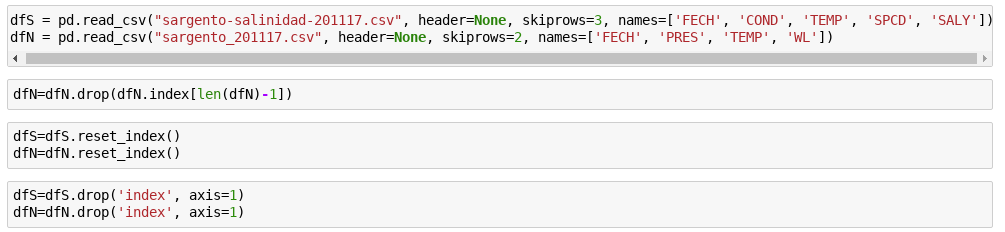
\includegraphics[width=12cm]{ElimDeRyC.png}
    
\end{center}
\vspace{0.2cm}

\subsection*{Act.2}
Antes de eliminar los renglones que no necesitaría, importe las bibliotecas de \textit{Numpy}, \textit{Pandas}, \textit{Seaborn}, \textit{matplotlib.pyplot} y \textit{datetime}.

\begin{verbatim}
import pandas as pd
import numpy as np
from datetime import datetime
import seaborn as sns
import matplotlib.pyplot as plt
\end{verbatim}

Después de importar las bibliotecas y de eliminar los renglones inservibles, utilice el comando \textit{DataFrame} para darles estructura a las tablas de datos. Luego me asegure que estos fueran del "tipo" indicado.

\begin{center}
	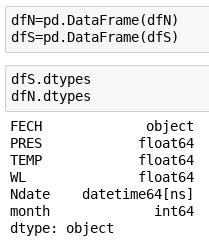
\includegraphics[width=4cm]{Dataframe.png}
    
\end{center}
\vspace{0.2cm}

\subsection*{Act.3}
Con la ayuda de la biblioteca \textit{Seaborn} cree diferentes graficas de caja (Boxplot) para diferentes variables.

\vspace{0.2cm}

Nota: en muchos casos se utilizaron dos temperaturas, una temperatura (Temperatura1) es la que aparece en el archivo llamado sargento-201117.csv, en el cual aparece la variable del nivel del mar. La otra (Temperatura2) aparece en el archivo llamado sargento-salinidad-201117.csv, en el cual aparece la variable de salinidad.

\begin{center}
	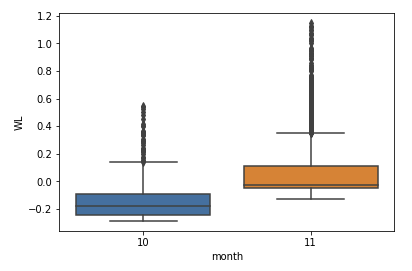
\includegraphics[width=8cm]{BxPltWL.png}
    
    Nivel del mar (m)
\end{center}
\vspace{0.3cm}

\begin{center}
	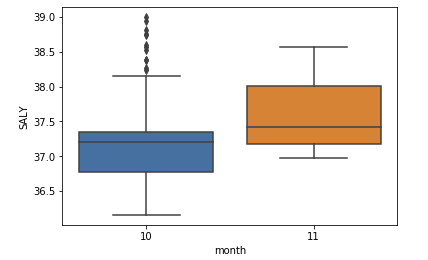
\includegraphics[width=8cm]{BxPltSALY.png}
    
    Salinidad (ppt)
\end{center}
\vspace{0.3cm}

\begin{center}
	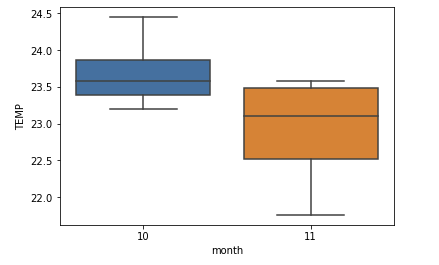
\includegraphics[width=8cm]{BxPltTEMPWL.png}
    
    Temperatura1 (C°) 
\end{center}
\vspace{0.3cm}

\begin{center}
	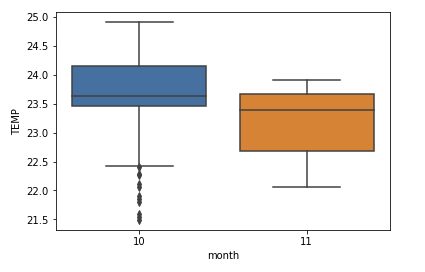
\includegraphics[width=8cm]{BxPltTEMPSALY.png}
    
    Temperatura2 (C°) 
\end{center}
\vspace{0.3cm}

Después de graficar, utiliza el comando \textit{describe} para obtener la mediana, media, los cuartiles, el máximo y el mínimo de los datos.

\begin{center}
	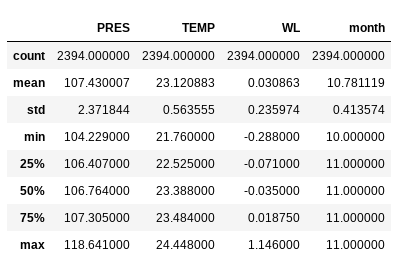
\includegraphics[width=8cm]{DescribeN.png}
    
    sargento-201117.csv
\end{center}
\vspace{0.3cm}

\begin{center}
	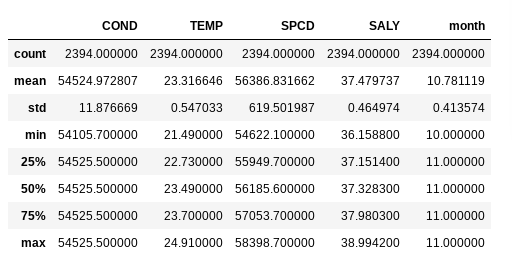
\includegraphics[width=8cm]{DescribeS.png}
    
    sargento-salinidad-201117.csv
\end{center}
\vspace{0.3cm}

\subsection*{Act.4}
Para esta parte, volvemos a utilizar \textit{Seaborn} para graficar los datos, solo que esta vez creamos una gráfica de regresión lineal con distribuciones marginales.

\begin{center}
	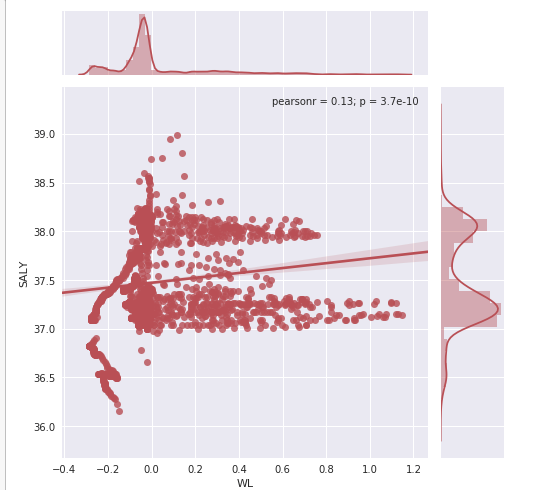
\includegraphics[width=10cm]{RegWLSALY.png}
    
    WL = Nivel del mar, SALY = Salinidad
\end{center}

\begin{center}
	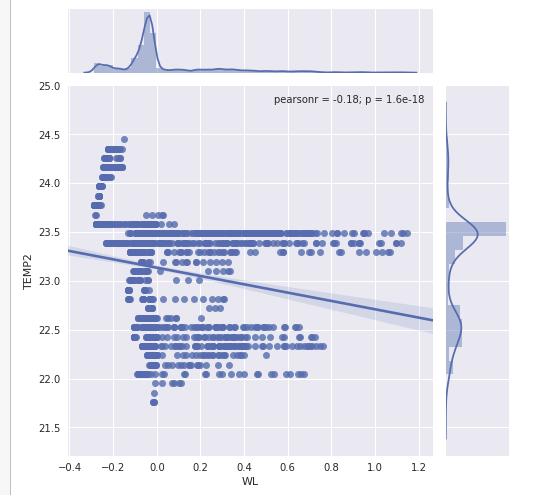
\includegraphics[width=10cm]{RegWLTEMP.png}
    
    WL = Nivel del mar, TEMP = Temperatura1
\end{center}
\vspace{0.3cm}

\begin{center}
	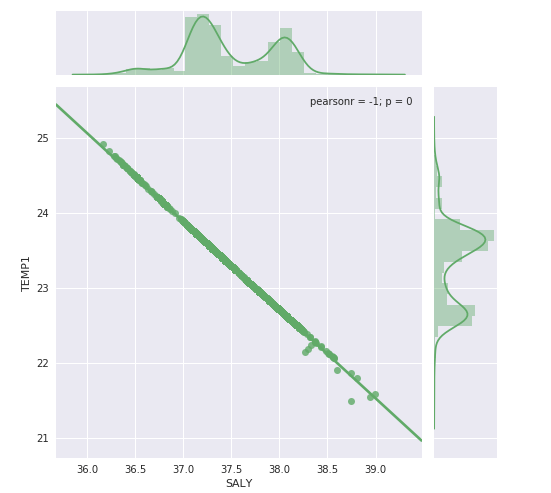
\includegraphics[width=10cm]{RegSALYTEMP.png}
    
    SALY = Salinidad , TEMP = Temperatura2
\end{center}
\vspace{0.2cm}

\subsection*{Act.5}
En esta parte utilizamos \textit{Matplotlib} para hacer tres graficas independientes de ciertas variables como función del tiempo.

\begin{center}
	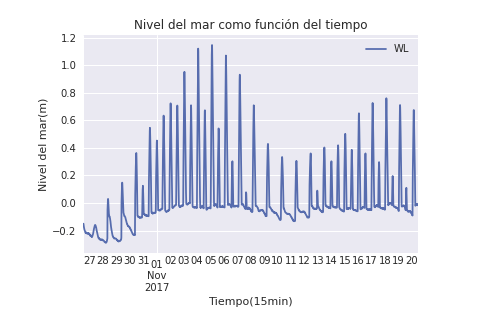
\includegraphics[width=12cm]{WLtime.png}
    
\end{center}
\vspace{0.3cm}

\begin{center}
	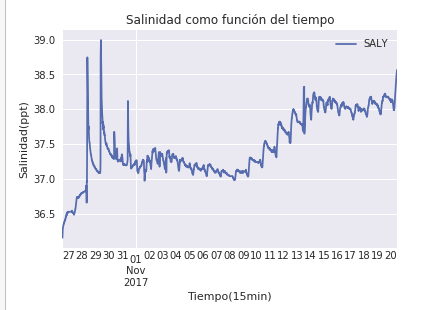
\includegraphics[width=12cm]{SALYtime.png}
    
\end{center}
\vspace{0.3cm}

\begin{center}
	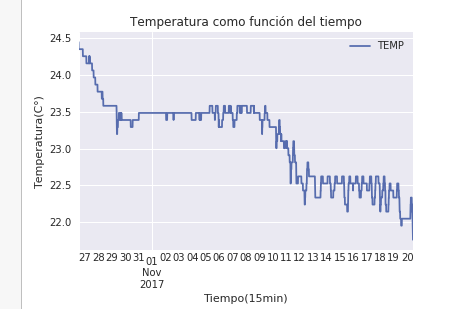
\includegraphics[width=12cm]{TEMPNtime.png}
      
\end{center}
\vspace{0.2cm}

\begin{center}
	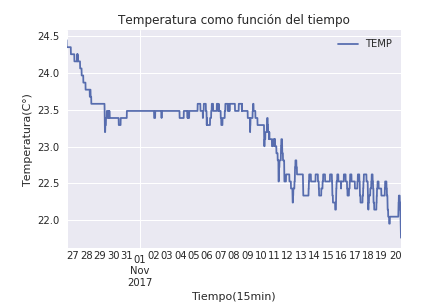
\includegraphics[width=12cm]{TEMPStime.png}
        
\end{center}
\vspace{0.2cm}

\subsection*{Act.6}
Esta parte es muy parecida a la parte anterior, solo que aquí hicimos graficas superpuestas con doble eje vertical. Estas graficas son muy útiles si quieres comparar dos variables y estas variables tienen rengos diferentes o una es simplemente mucho mayor o menor que la otra para poderlas comparar una encima de la otra de manera "normal".

\vspace{0.4cm}

\begin{center}
	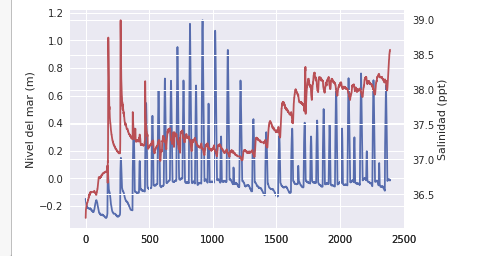
\includegraphics[width=10cm]{WL+SALY.png}
      
\end{center}
\vspace{0.2cm}

\begin{center}
	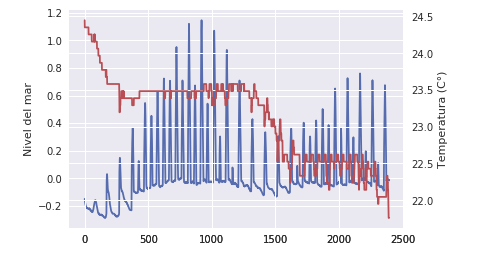
\includegraphics[width=10cm]{WL+TEMP.png}
        
\end{center}
\vspace{0.4cm}

Estas graficas también están en función del tiempo. En total hay 2394 datos, cada unidad en el eje x representa 15 minutos empezando del 26 de octubre a las 13:00 hasta las 11:15 del 20 de noviembre.

\subsection*{Act.7}
En esta actividad utilizamos las gráficas de la sección anterior, solo que tomamos un pequeño intervalo de tiempo de 5 días (480 unidades) para visualizar mejor la relación entre estas variables en función del tiempo.


Como se puede ver en el código, lo único que se le agrego a este fue \textit{plt.xlim([1000,1480])} para tomar datos que estuvieran prácticamente a la mitad de la lista.

\vspace{0.5cm}

\begin{verbatim}
from pylab import figure, show, legend, ylabel
 
# create the general figure
fig1 = figure()
 
# and the first axes using subplot populated with data 
ax1 = fig1.add_subplot(111)
line1 = ax1.plot(GRAF['WL'], 'b-')
ylabel("Nivel del mar (m)")
 
# now, the second axes that shares the x-axis with the ax1
ax2 = fig1.add_subplot(111, sharex=ax1, frameon=False)
line2 = ax2.plot(GRAF['SALY'], 'xr-')
ax2.yaxis.tick_right()
ax2.yaxis.set_label_position("right")
ylabel("Salinidad (ppt)")

plt.xlim([1000,1480])
show()
\end{verbatim}

\vspace{0.4cm}

\begin{center}
	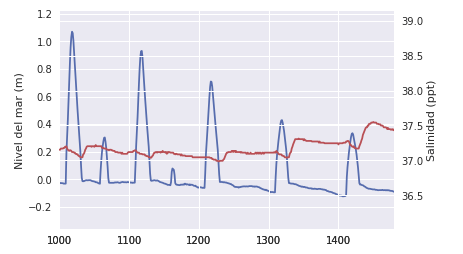
\includegraphics[width=11cm]{WL+SALY_lim.png}
      
\end{center}
\vspace{0.2cm}

\begin{center}
	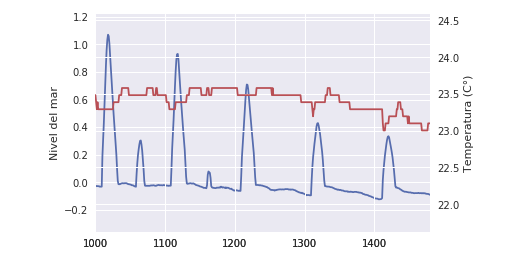
\includegraphics[width=12cm]{WL+TEMP_lim.png}
        
\end{center}
\vspace{0.5cm}

Analizando las gráficas uno puede observar que hay una ligera relación entre la temperatura y la salinidad con el nivel del mar.
Cuando el nivel del mar aumenta de manera considerable, la salinidad y la temperatura presentan una pequeña disminución.

\end{document}